\documentclass[a4paper]{article}


\usepackage{alphabeta} 
\usepackage{enumitem} 
\usepackage{mathtools}
\usepackage{amsmath, amssymb} 
\usepackage{amsthm}
\usepackage{cancel} 
\usepackage[margin=0.70in]{geometry} 
\geometry{left=2cm,right=2cm,top=2.4cm,bottom=2.4cm}	%the page geometry as defined, A4=210x297mm
\usepackage{graphicx}
\usepackage{wrapfig}
\usepackage[center]{caption}
\usepackage{textcomp}
\usepackage{tabto}
\usepackage{layout}
\usepackage{bm}
\usepackage{minipage-marginpar}
\usepackage[dvipsnames]{xcolor}
\usepackage{hyperref}
\usepackage{dutchcal}
\usepackage{derivative}
\usepackage{esint}
%\usepackage{biblatex}
\usepackage{subcaption}
\usepackage{fancyhdr}
\usepackage{booktabs}\usepackage{derivative}
\usepackage[flushleft]{threeparttable}
\usepackage[capbesideposition=outside,capbesidesep=quad]{floatrow}
\usepackage{derivative}
\usepackage[thinc]{esdiff}
\usepackage{lipsum}
\usepackage{arydshln}
%%RENEW

\newtheorem{problem}{Άσκηση}
\newtheorem*{solution*}{Λύση}
\newtheorem{definition}{Ορισμός}[subsection]
\newtheorem{properties}{Ιδιότητες}[subsection]
\newtheorem{theorem}{Θεώρημα}[subsection]
\newtheorem{protash}{Πρόταση}[subsection]
\newtheorem{porisma}{Πόρισμα}[subsection]
\newtheorem{lemma}{Λήμμα}[subsection]
\newtheorem*{prooof}{Απόδειξη}
\newtheorem*{notes}{Παρατηρήσεις}
\newtheorem*{note}{Παρατήρηση}
\newtheorem*{app}{Εφαρμογή} 
\newtheorem*{example}{Παράδειγμα}
\newtheorem*{examples}{Παραδείγματα}


\newcommand\numberthis{\addtocounter{equation}{1}\tag{\theequation}}
%\renewcommand{\labelenumi}{\roman{enumi}}
\newcommand{\approxtext}[1]{\ensuremath{\stackrel{\text{#1}}{\approx}}}
\renewcommand{\figurename}{Εικόνα.}
\renewcommand{\tablename}{Πίνακας.}
%\renewcommand\refname{New References Header}
\renewcommand*\contentsname{Περιεχόμενα}
%\DeclareDerivative{\odv}{\mathrm{d}}


\title{Σκέδαση Compton}
\author{Θωμόπουλος Σπυρίδων, ge19042}


\begin{document}
\pagestyle{fancy}
\fancyhead{}
\fancyfoot{}
\fancyhead[LO,LE]{\textbf{01 Σκέδαση Compton}}
\fancyfoot[CE,CO]{\thepage}

%\begin{titlepage}			%makes a title page. Remember to change the author, CID, username and group number to what is appropriate for you!
%	\centering
%	{\scshape\LARGE Εθνικό Μετσόβιο Πολυτεχνείο\par}
%	{\scshape \LARGE Σ.Ε.Μ.Φ.Ε.\par}
%	\vspace{1cm}
%	{\huge\bfseries Απορρόφηση Σωματιδίων β\par}
%	\vspace{1cm}
%	{\Large\itshape Θωμόπουλος Σπύρος\par}		%remember to change these!
%	
%	%		{\large Group \@group\unskip\strut\par}
%	{\large spyros.thomop@gmail.com/ ge19042@mail.ntua.gr\par \hfill \\}% 		%remember to change these!
%	\vspace{1cm}
%	{\large Ημερμονηνία Παράδοσης 17/05/2022\par}
%\end{titlepage}

\begin{titlepage}




\newcommand{\HRule}{\rule{\linewidth}{0.5mm}}

\includegraphics[width=8cm]{logo1.png}\\[1cm] 
\center 
\quad\\[1.5cm]
\textsl{\Large Εθνικό Μετσόβιο Πολυτεχνείο}\\[0.5cm] 
\textsl{\large Σχολή Εφαρμοσμένων Μαθηματικών και Φυσικών Επιστημών}\\[0.5cm] 
\makeatletter
\HRule \\[0.4cm]
{ \huge \bfseries \@title}\\[0.4cm] 
\HRule \\[1.5cm]
\begin{minipage}{0.4\textwidth}
\begin{flushleft} \large
\emph{Author:}\\
\@author 
\end{flushleft}
\end{minipage}
~
\begin{minipage}{0.4\textwidth}
\begin{flushright} \large

\end{flushright}
\end{minipage}\\[3cm]
\makeatother
%{\large An Assignment submitted for the UoS:}\\[0.5cm]
{\large \emph{Εργαστήριο Πυρηνικής Φυσικής \& Στοιχειωδών Σωματιδίων}}\\[0.5cm]
{\large \today}\\[2cm] 
\vfill 



\end{titlepage}

\subsection*{Σκοπός}
	Ο σκοπός της εν λόγω εργαστηριακής άσκησης είναι ο προσδιορισμός της εμβέλειας των σωματιδίων β με έναν καταμετρητή Geiger-Muller.
\subsection*{Θεωρητικά Στοιχεία}
	Το φαινόμενο Compton πρόκειται για την σκέδαση ενός φωτονίου ενέργειας Ε, σε ένα αρχικά ακίνητο ηλεκτρόνιο.
	Μετά την αλληλεπίδραση, το φωτόνιο αποκτά ενέργεια Ε' και κινείται σε γωνία θ προς την αρχική κατεύθυνση και το ηλεκτρόνιο $E_{e}'$ σε γωνία φ, όπως φαίνεται στην Εικόνα (\ref{fig1}). 
	\begin{figure}[h!]
		\centering
		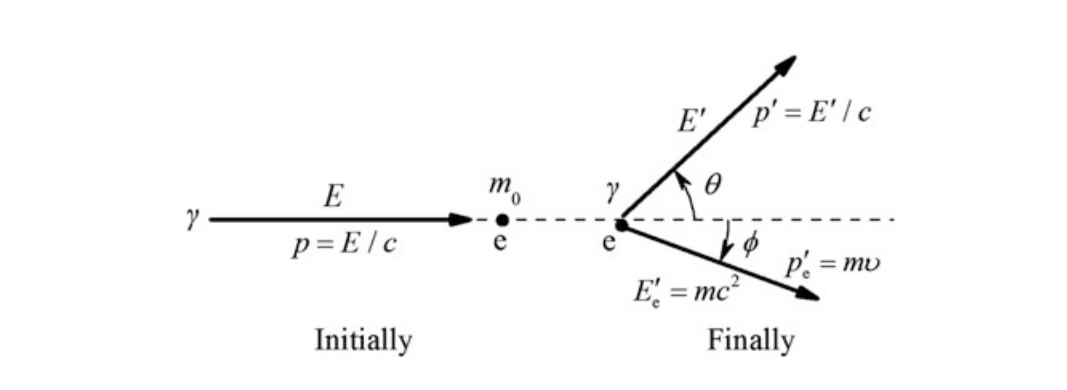
\includegraphics[scale=0.5]{compton.png}
		\caption{Σκέδαση Compton}
		\label{fig1}
	\end{figure}
	
	Στον παρακάτω Πίνακα φαίνονται τα στοιχεία των τετραορμών των σωματιδίων πριν και μετά την σκέδαση.
	\begin{table}[h!]
		\centering 
		\begin{tabular}{c|c|c}
					 & Πριν  & Μετά \\\hline
			$\gamma$ & $p_\gamma=(E,\bm{p_\gamma})$ &  $p_\gamma'=(E', \bm{p_\gamma'})$ \\
			e        & $p_e     =(m_e,0)$                &  $p_e'=(E_e', \bm{p_e'})$
		\end{tabular}
		\label{tab}
	\end{table}
	
	Από διατήρηση της τετραορμής έχουμε ότι 
	\begin{align*}\label{eq1}
		p_\gamma + p_e = p_\gamma'+p_e  \numberthis
	\end{align*}
	Στην οποία περιέχεται η διατήρηση της ενέργειας
		\begin{align*}\label{eq2}
			E +m_e = E' + E_e' \numberthis
		\end{align*}
	και της ορμής 
		\begin{align*}\label{eq3}
			\bm{p_\gamma} = \bm{p_\gamma'} + \bm{p_e'} \numberthis
		\end{align*}
	
	Από την εξίσωση (\ref{eq2}) έχουμε ότι 
		\begin{align*}\label{eq4}
			|\bm{p_e'}|^2 =&  |\bm{p_\gamma'} -\bm{p_\gamma}  |^2 \xRightarrow{E^2=p^2+m^2}\\
			E_e'^2 - m_e^2      =& |\bm{p_\gamma}'|^2 +|\bm{p_\gamma}|^2 -2\bm{p_\gamma}\cdot\bm{p_\gamma'}\Rightarrow\\
			(E-E'+m_e)^2-m_e^2  =& E'^2 + E^2 - 2EE'cos\theta \Rightarrow\\
			 \cancel{E^2} + \cancel{E'^2}+\cancel{m_e^2} + 2Em_e -2E'm_e -2EE' - \cancel{m_e^2}   =& \cancel{E^2} + \cancel{E'^2}-2EE'cos\theta \Rightarrow\\
			 m_e(E-E')    =& EE'(1-cos\theta) \Rightarrow\\
			    \frac{1}{E'} - \frac{1}{E} =& \frac{1-cos\theta}{m_ec^2}\numberthis
		\end{align*}
		
		
Από την παραπάνω σχέση προκύπτει πως η μέγιστη ενέργεια, άρα και κινητική ενέργεια) του ηλεκτρονίου επιτυγχάνεται όταν η Ε' είναι ελάχιστη, δηλαδή όταν το 1/Ε' είναι μέγιστο, δηλαδή από την σχέση (\ref{4}) όταν $\theta = \pi$. Έχουμε 
	\begin{align*}\label{eq5}
		T_e^{max} =& m_e(\gamma_{Lor.} -1)c^2 \Rightarrow\\
				  =& m_e\gamma_{Lor.}c^2 - m_ec^2 \Rightarrow\\
				  =& E_e'-m_ec^2 \xRightarrow{(\ref{eq2})}\\ 
		          =& E - E' \numberthis
	\end{align*}
	
Λύνουμε την εξίσωση (\ref{eq4}) προς E'  
	\begin{align*}\label{eq6}
		1/E' =& \frac{m_ec^2 + E- Ecos\theta}{Em_ec^2} \xRightarrow{\theta=\pi}\\
			 =& \frac{m_ec^2 +2E }{m_ec^2E} \Rightarrow\\
		E'   =& \frac{Em_ec^2}{m_ec^2 + 2E}	 	 \numberthis
	\end{align*}
	Αντικαθιστώντας την (\ref{eq6}) στην (\ref{eq5}) παίρνουμε την μέγιστη κινητική ενέργεια που μπορεί να έχει το ηλεκτρόνιο συναρτήσει της αρχικής ενέργειας του φωτονίου
	\begin{align*}\label{eq7}
		T_e^{max} =& E - \frac{Em_ec^2}{m_ec^2 + 2E}\Rightarrow\\
		          =& \frac{2E^2}{m_ec^2 + 2E} \numberthis
	\end{align*}
	
Αν την λύσουμε ως προς την μάζα του ηλεκτρονίου παίρνουμε ότι 
	\begin{align*}\label{eq8}
		 m_ec^2 =& \frac{2E(E-T_e^{max})}{T_e^{max}} \numberthis
	\end{align*}
	
		Η πειραματική εκδήλωση του παραπάνω αποτελέσματος θα είναι αντιληπτή ως μία σχετικά απότομη μείωση στο φάσμα Compton, δηλαδή στο διάγραμμα Counts-Ενέργεια ανιχνευόμενων φωτονίων. Αυτό θα συμβαίνει διότι από την μέγιστη αυτή ενέργεια και μετά τα φωτόνια θα δίνουν το μεγαλύτερο μέρος της ενέργειάς τους στα ηλεκτρόνια επομένως εμείς θα ανιχνεύουμε λιγότερα φωτόνια υψηλής ενέργειας.
	
	
	Ο πειραματικός τρόπος με τον οποίο θα δημιουργήσουμε καταστάσεις που θα συμβαίνουν κρούσεις Compton είναι μέσω ραδιενεργών πηγών. Αυτές καθώς αποδιεγείρονται θα εκπέμπουν ακτίνες γ. Με την σειρά τους οι γ μπορούν να αλληλεπιδράσουν με ένα υλικό μέσω τριών τρόπων, με φωτοηλεκτρικο΄, με Compton και με δίδυμη γέννεση. Καθένας από αυτούς έχει ως αποτέλεσμα την δημιουργία τελικών ελεύθερων ηλεκτρονίων, είτε από ιονισμό είτε από δημιουργία ζεύγους $e^-e^+$.
	
	
	Τα εν λόγω ηλεκτρόνια θα κινούνται εντός ενός κρυσταλλικού υλικού όπου και θα χάνουν ενέργεια ακολουθώντας την καμπύλη Bethe-Bloch.  Έτσι, ιονίζοντας τα άτομα του πλέγματος θα παράγονται εκ νέου φωτόνια λόγω της αποδιέγερσης των ατόμων. Αυτά επειδή θα είναι χαμηλότερης ενέργειας ( ορατή περιοχή ) δεν θα ιονίζουν περεταίρω τα άτομα και θα οδηγούνται μέσω μίας οπτικής κοιλότητας σε έναν φωτοπολλαπλασιαστή δημιουργώντας μικρούς παλμούς ρεύματος οι οποίοι εν τέλει προστίθενται και δίνουν τον συνολικό.
	
	Ακόμη, στο φάσμα μας θα υπάρχουν και κάποια άλλα σημεία ενδιαφέροντος πέρα από την απότομη μείωση που θα αναδεικνύει το φαινόμενο Compton. 
	Το ένα από αυτά πρόκειται για μία κορυφή σε  μεγαλύτερη ενέργεια και πρόκειται για τα φωτόνια που δεν έχουν αλληλεπιδράσει και τα ανιχνεύουμε απ' ευθείας από την πηγή.
	Ακόμη, θα ανιχνεύουμε μία κορυφή σε πολύ χαμηλές ενέργειες ($E_X$) που προέρχεται από τον θυγατρικό πυρήνα και είναι ακτίνες Χ και μία άλλη κορυφή σε ενδιάμεση ενέργεια που προέρχεται από τις ακτίνες γ που αλληλεπιδρούν με ατομικά ηλεκτρόνια που οπισοσκεδάζονται διαφεύγοντας από το υλικό ($E_{BS}$). 
	
	Οι δύο περιοχές που σχετίζονται άμεσα με το φαινόμενο Compton είναι συμμετρικές, με την έννοια ότι στην περιοχή απότομης μείωσης της ενέργειας έχουμε οπισθοσκέδαση και διαφυγή του φωτονίου ενώ στην δεύτερη περίπτωση της κορυφής έχουμε οπισθοσκέδαση και διαφυγή του ηλεκτρονίου.
	Γενικά θα ισχύει ότι  
		\begin{align*}\label{eq9}
			E_\gamma = E_{BS} + T^e_{max} \numberthis
		\end{align*}
		
\subsection*{Πειραματική Διάταξη}
	Η πειραματική Διάταξη αποτελείται από 
		\begin{itemize}
			\item[.]  Κρύσταλλο NaI 
			\item[.]  Φωτοπολλαπλασιαστή 
			\item[.]  H/Y για την λήψη του φάσματος (1024 κανάλια)
			\item[.]  Ραδιενεργό Πηγή $^{22}Na$ για calibration
			\item[.]  Ραδιενεργές Πηγές $^{54}Mn, ^{137}Cs, ^{66}Co $ για μετρήσεις
		\end{itemize}
		
		Σε κάθε κανάλι του αναλυτή αντιστοιχεί μία τιμή της ενέργειας με την λογική ότι η ενέργεια αυξάνεται στα μεγαλύτερα κανάλια. Θα χρειαστεί να κάνουμε βαθμονόμηση των καναλιών χρησιμοπιοιώντας ραδιενεργές πηγές που εκπέμπουν ακτινοβολία σε γνωστή ενέργεια.
		
		Καθώς ένα φωτόνιο γ εισέλθει στο αριστερό μέρος του ανιχνευτή NaI στο οποιο είναι τοποθετημένος ο κρύσταλλος NaI (Περιοχή Ι), διεγείρει τα ηλεκτρόνια του NaI, με αποτέλεσμα την εκπομπή φωτονίων στο ορατό, τα οποία διαφεύγουν και εισέρχονται στην Περιοχή ΙΙ. Εκεί υπάρχει αρχικά μία φωτοκάθοδος η οποία εκπέμπει ηλεκτρόνια όταν προσπίπτουν πάνω της τα φωτόνια που δημιουργούνται στην Περιοχή Ι. Έπειτα τα ηλεκτρόνια κατευθύνονται με την βοήθεια ενός ηλεκτρικού πεδίου προς την πρώτη δύνοδο (dynode) η οποία βρίσκεται σε ένα θετικό δυναμικό και είναι επικαλυμμένη με κάποιο υλικό που εκπέμπει δευτερεύοντα ηλεκτρόνια (π.χ. BeO, MgO, GaP κλπ). Έπειτα αυτά κατευθύνονται προς μία άλλη δύνοδο που βρίσκεται σε πιο θετικό δυναμικό κ.ο.κ. Μπορούμε να πετύχουμε ενίσχυση κατά 10 φορές σε κάθε στάδιο. Εν τέλει, τα ηλεκτρόνια καταλήγουν στο τέλος της Περιοχής ΙΙ σε μία άνοδο όπου με έναν Analog to Digital Converter (ADC) παίρνουμε ψηφιακό σήμα το ύψος του οποίου αντιστοιχεί σε μία ενέργεια, άρα σε ένα κανάλι.
	
	\begin{figure}[h!]
		\centering
		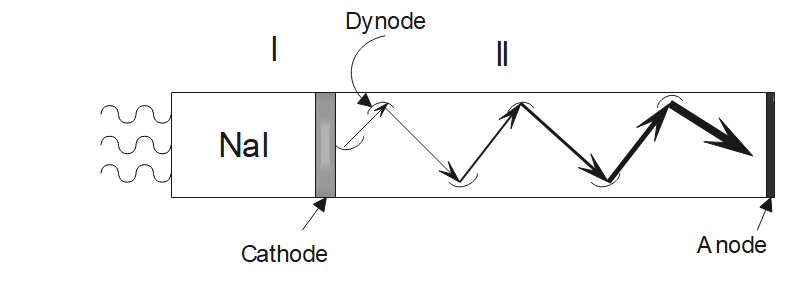
\includegraphics[scale=0.5]{ph_mult.png}	
		\caption{Βασική Λειτουργία του Φωτοπολλαπλασιαστή}
		\label{fig2}
	\end{figure}			
	
\subsection*{Πειραματική Διαδικασία - Επεξεργασία Μετρήσεων}
	Χρησιμοποιώντας πηγή $^{22}Na$ βαθμονομούμε τον ανιχνευτή μας. Δηλαδή αφού πάρουμε το φάσμα του $^{22}Na$ και δεδομένου ότι γνωρίζουμε τις τιμές της ενέργειας σε τρια χαρακτηριστικά σημεία ( στην κορυφή μέγιστης ενέργειας, στην κορυφή BS και στο ενδιάμεσο Compton Edge) μπορούμε να αντιστοιχίσουμε γραμμικά ένα κανάλι σε μία ενέργεια.
	Αφού κάνουμε αυτό, είμαστε έτοιμοι για να προχωρήσουμε στην καταγραφή των φασμάτων των υπολοίπων πυρήνων. 
	
	Στον Πίνακα (\ref{mat1}) φαίνονται οι ενέργειες της κορυφής από τα απευθείας φωτόνια $E_\gamma$, του σημείου στο Compton Edge $T^e_{max}$( μεσαίο κανάλι του διαστήματος πτώσης του φάσματος ) και την ενέργεια που αντιστοιχεί στην οπισθοσκέδαση του φωτονίου $E_{BS}$.
	Επίσης στον Πίνακα (\ref{mat1}) φαίνεται το άθροισμα $T^e_{max} + E_{BS}$ τα οποίο θεωρητικά θα πρέπει να είναι ίσο με την $E_\gamma $ καθώς και σχετική του απόκλιση από αυτή.
	
	\begin{table}[h!]
		\centering 
		\begin{tabular}{c|c|c|c||c|c}
			Πηγή       & $E_\gamma(keV)$  &  $T^e_{max}(keV)$  & $E_{BS}(keV)$ & $T^e_{max}(keV)+E_{BS}$  & $\Delta E = (E_\gamma - T^e_{max}-E_{BS})/E_\gamma$ \\\hline 
			$^{54}Mn$  & 849.9             &     602.2     & 139.3 & 108.4& 13\%\\  
			$^{137}Cs$ & 669.5             &     485.5     & 126.5 & 57.5&8\%\\ 
			$^{66}Co $ & $\underbrace{1235.6}_{M.Τ. 1167.5 \& 1303.7}$ &     967.9     & 155.7 & 112.0 & 9\% \\ 
			         %  & 1303.7           &               & 
		\end{tabular}
		\caption{Πειραματικές Μετρήσεις \& έλεγχος της σχέση (\ref{eq9})\\ \textcolor{red}{!**!} Το $^{66}Co$ εκπέμπει σε δύο κορυφές ακτίνες γ οι οποίες μετρήθηκαν 1167.5 \& 1303.7keV. Γι' αυτό θα χρησιμοποιηθεί η Μέση Τιμή τους που είναι 1265.6keV}
		\label{mat1}
	\end{table}
	
	\subsubsection*{Υπολογισμός Μάζας Ηλεκτρονίου}
	Έχει αποδειχτεί στο κομμάτι της θεωρίας πως ισχύει (\ref{eq8}) 
	\begin{align*}
		m_ec^2 =& \frac{2E(E-T_e^{max})}{T_e^{max}}
	\end{align*}
	όπου $E=E_\gamma$ είναι η αρχική ενέργεια του φωτονίου γ, δηλαδή η ενέργεια στην οποία αντιστοιχεί η υψηλότερη κορυφή και $T_e^{max}$ είναι η μέγιστη κινητική ενέργεια που μπορεί να αποκτήσει το ηλεκτρόνιο. Όλες αυτές οι τιμές υπάρχουν στον Πίνακα (\ref{mat1}), συνεπώς μπορούμε να υπολογίσουμε την μάζα του ηλεκτρονίου από κάθε πηγή ξεχωριστά και για τους μετέπειτα υπολογισμούς μας να χρησιμοποιήσουμε την μέση τιμή αυτών.
	
	Τα αποτελέσματα για τις μάζες καθώς και των αποκλίσεών τους από την αναμενόμενη 511keV φαίνονται στον Πίνακα (\ref{mat2}) 
	\begin{table}
			\centering 
			\begin{tabular}{c|c|c}
					Πηγή & $m_e(keV/c^2)$ & $\delta m_e= (m_{bib}-m_e)/m_{bib}$ \\ \hline
					$^{54}Mn $ & 700 & 37\%\\
					$^{137}Cs$ & 508 &  7\%\\
					$^{66}Co $ & 684 &  34\%\\
			\end{tabular}
			\caption{Τιμές για την Μάζα}
			\label{mat2}
		\end{table}	
	Άρα η μέση τιμή της μάζας είναι 
		\begin{align*}
			m_e = (630\pm87)keV/c^2 \numberthis
		\end{align*}
	Όπως βλέπουμε ένα ένα σχετικό σφάλμα της τάξης του 23\% από την αναμενόμενη το οποίο είναι πολυ μεγάλο.
	
	\subsubsection*{Υπολογισμοί για Ενέργειες}
	Γνωρίζουμε ότι ισχύει 
	\begin{align*}
		E_e =& m_0\gamma c^2 = \underbrace{m_0(\gamma-1)c^2}_{T_e} + \underbrace{m_0c^2}_{E_0} \Rightarrow\\
		    =& T_e^{max} + E_0 
	\end{align*}
	Άρα χρησιμοποιώντας την παραπάνω σχέση μπορούμε να υπολογίσουμε την συνολική Σχετικιστική Ενέργεια του ηλεκτρονίου. Έπειτα διαιρώντας με την ενέργεια ηρεμίας μπορούμε να βρούμε τον παράγοντα Lorentz $\gamma = E_e/m_0c^2$. 
	
	Από τον ορισμό του γ βρίσκουμε την ταχύτητα του ηλεκτρονίου $\beta = \sqrt{(\gamma^2-1)/\gamma^2}$.
	Τέλος, για σύγκριση μπορούμε να υπολογίσουμε την κλασική τιμή της κινητικής ενέργειας των ηλεκτρονίων $T_{e,clas} = 1/2 m_0 c^2\beta^2$. 
	Τα παραπάνω μεγέθη φαίνονται όπως προκύπτουν ξεχωριστά για κάθε πηγή στον παρακάτω Πίνακα (\ref{mat3}) 
	\begin{table}[h!]
		\centering 
		\begin{tabular}{c|c|c|c|c||c}
				  Πηγή & $E_e(keV)$  & $\gamma$ & $\beta$ & $T_{e,class}(keV)$ & $T_e^{max}(keV)$\\\hline
			$^{54}Mn $ & 1301        &   1.86  &   0.0.680& 162 &602\\
			$^{137}Cs$ & 993		    &   1.96  &    0.699 & 124 &486\\
 			$^{66}C0 $ & 1651        &  2.42  &    0.766 & 200 & 968
		\end{tabular}
		\caption{Μεγέθη υπολογισμένα για κάθε πηγή }
		\label{mat3}
	\end{table}
	Φαίνεται ξεκάθαρα πως η κλασικά υπολογισμένη κινητική ενέργεια έχει μεγάλη απόκλιση από την πειραματική στην οποία πρέπει να συνυπολογιστούν και σχετικιστικές διορθώσεις. 
	
	Τέλος σχεδιάζονται οι γραφικές παραστάσεις της ολικής σχετικιστικής ενέργειας, της σχετικιστικής κινητικής ενέργειας και της κλασικής κινητικής ενέργειας σύμφωνα με τις σχέσεις 
	\begin{align*}
		 E_{e,total} =& m_0 c^2 \gamma \\
		 T_{e}   =& (\gamma-1)m_0c^2 \\
		 T_{e,class} =& \frac{1}{2}m_0c^2 \beta^2
	\end{align*}
	
	\begin{figure}[h!]
		\centering
		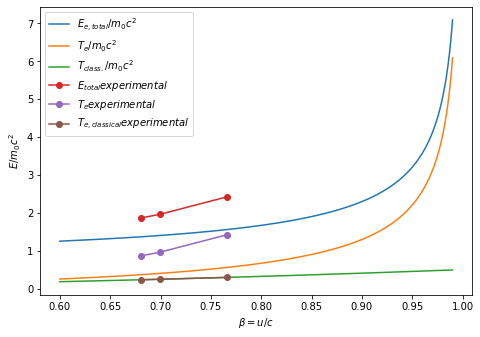
\includegraphics[scale=0.7]{energy_plots}
		\caption{Ολική και Κινητική Σχετικιστική και Κλασική Κινητική Ενέργεια συναρτήσει του β, όπου $m_0$ η πειραματική τιμή}
		\label{fig3}
	\end{figure}
	

\subsection*{Συμπεράσματα}
	Εν τέλει τα αποτελέσματά μας είναι ποιοτικά όπως αναμέναμε, δηλαδή υπάρχει ασυμφωνία της κινητικής ενέργειας με την μη σχετικιστική θεώρηση. Ωστόσο, οι ποσοτικοί υπολογισμοί δεν ήταν ιδιαίτερα ακριβείς καθώς είχαμε αποκλίσεις έως και $~30\%$ από τα βιβλιογραφικά δεδομένα για την μάζα του ηλεκτρονίου.
\end{document}